\documentclass{Handbuch}
\usepackage{graphicx} 
\usepackage{hyperref}
\begin{document}
\parindent 0pt
\newgeometry{top=2.5cm,bottom=2.0cm,left=2.5cm,right=2.5cm} % Befehl wird nur benötigt, falls Änderungen an den Seitenrändern in der Datei "Vorlage.cls" vorgenommen werden.

\begin{titlepage}

\titelseite{Softwaretechnik}{Fakultät für Informatik und Elektrotechnik}

\vspace*{6cm}

\BAtitel{Nutzerhandbuch}{Projekt Softwaretechnik WS 18/19}

\vspace{1cm}

\begin{table}[h]
\onehalfspacing
\begin{tabular}{p{5cm}|p{0.1cm} p{10cm}l}
\textsc{Projektmitglieder} & & \textsc{Kristi Bartelt}\\
\textsc{} & & \textsc{Sebastian Beleites}\\
\textsc{} & & \textsc{Diana Bürger}\\
\textsc{} & & \textsc{Sven Hagemann}\\
\textsc{} & & \textsc{Christoph Häseker}\\
\textsc{} & & \textsc{Oleg Mayer}\\
\textsc{Abgabe:} & & \textsc{\today}\\
\end{tabular}
\end{table}
\end{titlepage}

\restoregeometry

\pagenumbering{Roman} % \pagenumbering{roman} = Kleinschreibung: II -> ii.

\tableofcontents % Inhaltsverzeichnis.

\newpage % Neue Seite.

\pagenumbering{arabic} % Ab hier folgt die arabische Seitennummerierung.


%%%%%%%%%%%%%%%%%%%%%%%%%%%%%%%%%%%%
\section{Einleitung}
Dieses Nutzerhandbuch soll eine Orientierung in der Software und die einfache Bedienung für Nutzer ermöglichen.

\subsection{Zielbestimmung}
Die Lehrstühle der Universität Rostock sollen durch das Produkt in der Lage sein, die im Zusammenhang mit den Lehrveranstaltungen notwendigen Verwaltungsaktivitäten durch eine Software zu verwalten.

\subsection{Nutzerrollen}
Es gibt die drei Nutzerrollen Administrator, Dozent und Student, welche jeweils eine verschiedene Ansicht auf die Software haben.
Der Administrator muss die Veranstaltung für einen Lehrstuhl, der die Software nutzen möchte, initial eintragen und die zuständigen Dozenten festlegen.
Alle weiteren Einstellungen und die Verwaltung der Übungsgruppen, Projektteams usw. werden von den Dozenten vorgenommen.
Studenten können sich mit der Software in Übungsgruppen und Projektteams einschreiben und ihre erreichten Leistungen einsehen.


%%%%%%%%%%%%%%%%%%%%%%%%%%%%%%%%%%%%
\newpage
\section{Installation}
\subsection{Installationsanleitung für die Benutzung des SWT Programms (Client)}
Das SWT-Programm wurde nur in der Java Version 12 getestet.\\
Um Java auf Ihrem System zu installieren, gehen Sie auf die Seite: \url{<https://www.oracle.com/technetwork/java/javase/downloads/index.html>}.\\
Dort können Sie sich Java in der Version 12 für Ihr System herunterladen.\\
Eine Installationsanweisung für verschiedene Betriebssysteme finden Sie hier:\\
\url{<https://docs.oracle.com/en/java/javase/12/install/overview-jdk-installation.html#GUID-8677A77F-231A-40F7-98B9-1FD0B48C346A>}\\

Nachdem Sie Java erfolgreich installiert haben, können Sie das SWT-Programm starten.

\subsection{Installationsanleitung für Server/Datenbank}
Vorausgesetzt wird Ubuntu Version 18.04 oder eine ähnliche Linux Umgebung.\\

Alle benötigten Komponenten können aus den offiziellen Paketquellen installiert werden.\\

Öffnen Sie einen Browser und Laden sie sich \url{https://github.com/ufgdcx/Uni_Softwaretechnik.git} herunter.\\
Öffnen Sie eine Konsole und installieren sie Folgende Pakete:\\

\$ sudo apt-get install apache2 libapache2-mod-php7.2 php7.2 php7.2-mysql mysql-server\\

Für einen ersten Test, öffnen Sie mit einem Webbrowser die Internet-Adresse \url{http://localhost}.\\
Dort sollte Folgendes zu lesen sein:\\

	It works!\\
	This is the default web page for this server.\\
	The web server software is running but no content has been added, yet.\\

Wenn diese Seite nicht angezeigt wird, wurde Apache vermutlich noch nicht gestartet. In diesem Fall starten Sie den Webserver mit folgendem Befehl:\\

\$ sudo service apache2 start\\

Im Verzeichnis /var/www/html/ sollten Sie nun eine Datei erstellen mit dem Namen phpinfo.php mit folgendem Inhalt:\\

\textless ?php\\
phpinfo();\\
?\textgreater \\

Rufen Sie anschließend mit dem Webbrowser sie Adresse: \url{http://localhost/phpinfo.php} bzw. \url{http://IP-ADRESSE/phpinfo.php}
auf. Dort sollten nun alle Informationen zur verwendeten PHP-Version stehen.\\

Nun öffnen Sie eine Konsole und installieren sie Folgendes Paket:\\

\$ sudo apt-get install phpmyadmin\\

Nachdem Sie phpmyadmin erfolgreich eingerichtet haben, rufen Sie mit dem Webbrowser die Adresse: \\
\url{http://localhost/phpmyadmin} bzw. \url{http://IP-ADRESSE/phpmyadmin} auf.\\

Loggen Sie sich mit dem Username root und dem entsprechenden Passwort ein.\\
Klicken Sie nun auf \frqq User accounts\flqq{} und dann auf \frqq Add user account\flqq{} und legen Sie sich einen neuen User mit folgenden Informationen an:\\

Login Information:\\
- User name: swt\\
- Host name: Any host\\
- Password: swt123456\\
- Authentication Plugin: Native MySQL authentication\\

und setzen Sie ein Haken unter \frqq Database for user account\flqq{} bei \frqq Create database with same name and grant all privileges\flqq.\\

Anmerkung: Sie können natürlich auch ein anderen Username wählen mit einem anderen Passwort.\\

Loggen Sie sich als Root aus und mit Ihrem neu erstellten User swt ein.\\
Klicken Sie auf die swt Database und dann auf \frqq Import\flqq. Klicken Sie auf \frqq Browse...\flqq{} und navigieren sie zu dem am Anfang heruntergeladenen git Repository unter .../Uni\_Softwaretechnik/Datenbank/swt\_datenbank.sql. Klicken Sie anschließend auf \frqq Go\flqq{} und die Datenbank wird geladen.\\

Anschließend müssen Sie noch in .../Uni\_Softwaretechnik/src/Database/DataSourceConn.java die Verbindungsdaten entsprechend ändern.



%%%%%%%%%%%%%%%%%%%%%%%%%%%%%%%%%%%%
\newpage
\section{Adminhandbuch}

\subsection{Starten der Anwendung}
Wenn Sie die Anwendung gestartet haben, erscheint ein Fenster mit allen derzeitig verfügbaren Veranstaltungen.
\begin{center}
	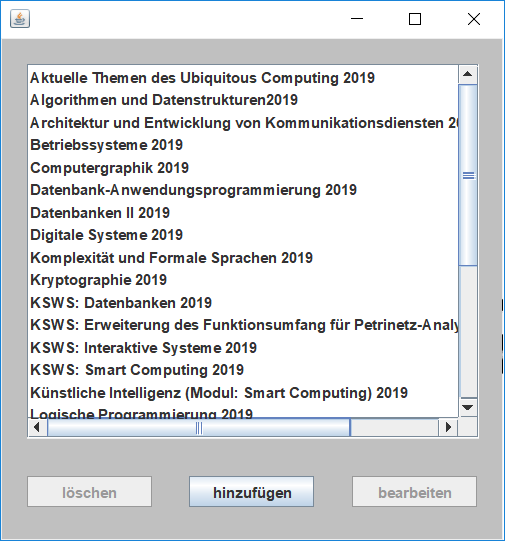
\includegraphics[width=0.7\textwidth]{img_adminGUI_01.png}
\end{center}
\subsection{Veranstaltung hinzufügen}
Um eine Veranstaltung zu der Veranstaltungsliste hinzuzufügen, klicken Sie auf \frqq hinzuf...\flqq{}.
Danach erscheint ein neues Fenster mit den Informationen über die zu erstellende Veranstaltung.
\begin{center}
	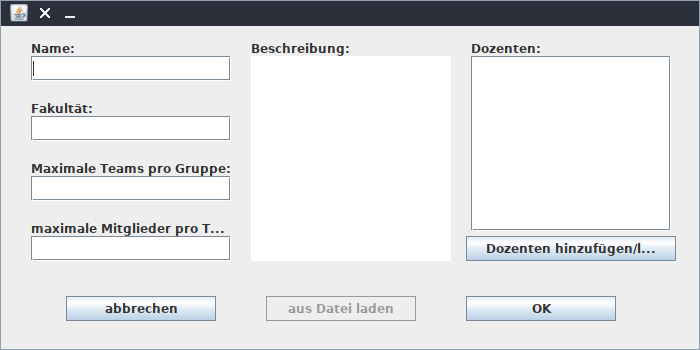
\includegraphics[width=0.7\textwidth]{img_adminGUI_02.png}
\end{center}
Dort können Sie Ihre Informationen eintragen.
\begin{center}
	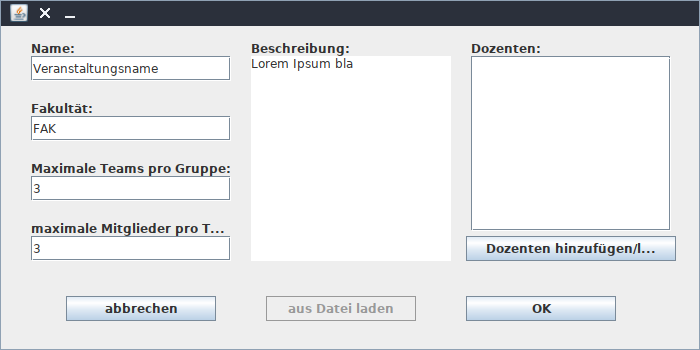
\includegraphics[width=0.7\textwidth]{img_adminGUI_03.png}
\end{center}
Um der Veranstaltung Dozenten zuzuweisen, klicken Sie auf \frqq Dozenten hinzufügen/l...\flqq{}.
Danach erscheint ein neues Fenster mit allen Dozenten, die man der Veranstaltung hinzufügen kann auf der linken Seite und einer Liste mit allen Dozenten, die der Veranstaltung zugeordnet worden sind auf der rechten Seite. Da wir eine neue Veranstaltung erstellt haben ist die rechte Liste natürlich noch leer.
\begin{center}
	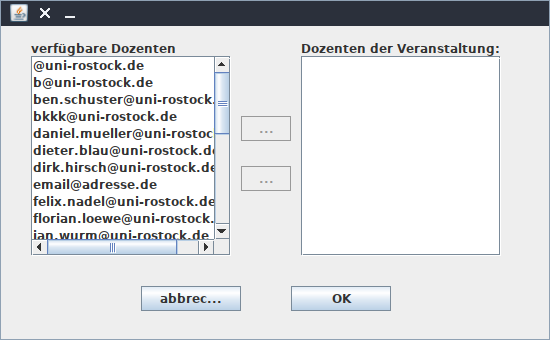
\includegraphics[width=0.7\textwidth]{img_adminGUI_04.png}
\end{center}
Um einen verfügbaren Dozenten zu der neu erstellten Veranstaltung hinzuzufügen klicken sie auf den gewünschten Dozenten in der linken Liste und dann auf den oberen der beiden Buttons zwischen der rechten und linken Liste.
\begin{center}
	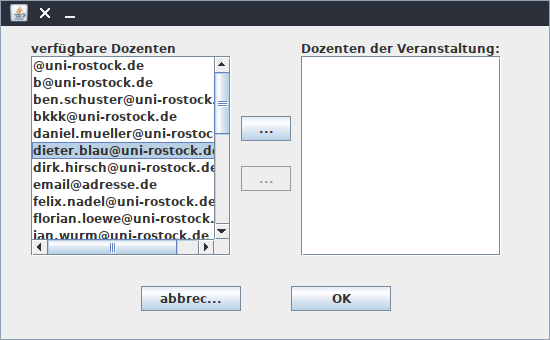
\includegraphics[width=0.7\textwidth]{img_adminGUI_05.png}
\end{center}
Jetzt wurde der Dozent zu der neuen Veranstaltung hinzugefügt. Damit wurde er auch aus der Liste, der für diese Veranstaltung zur Verfügung stehenden Dozenten, entfernt. Beachten Sie aber, dass ein Dozent natürlich mehreren (verschiedenen) Veranstaltungen zugeordnet sein kann.
\begin{center}
	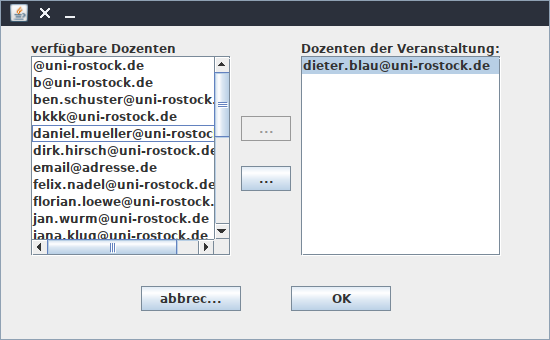
\includegraphics[width=0.7\textwidth]{img_adminGUI_06.png}
\end{center}
Mit \frqq OK\flqq{} bestätigen sie Ihre Auswahl und gelangen zurück zum vorherigen Fenster, in der nun die Dozenten in der Dozentenliste eingetragen worden sind.
\begin{center}
	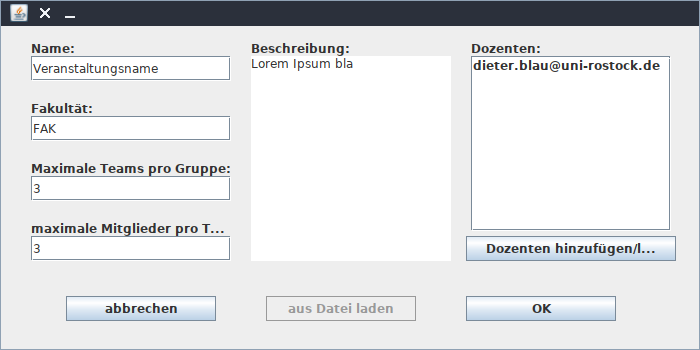
\includegraphics[width=0.7\textwidth]{img_adminGUI_07.png}
\end{center}
Bestätigen Sie Ihre Eingaben, indem Sie auf \frqq OK\flqq{} klicken, und Sie gelangen wieder zur Übersicht aller Veranstaltungen. In dieser Liste steht nun die gerade neu erstellte Veranstaltung.
\begin{center}
	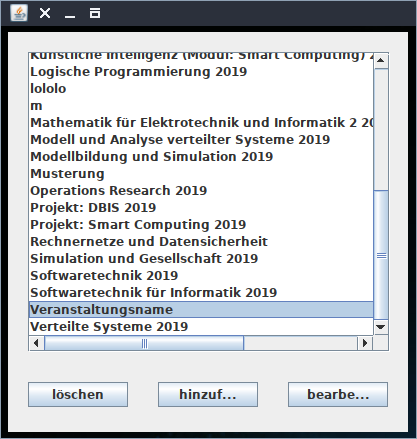
\includegraphics[width=0.7\textwidth]{img_adminGUI_08.png}
\end{center}

\subsection{Veranstaltung bearbeiten}
Falls Sie eine Veranstaltung überarbeiten möchten, können Sie die entsprechende Veranstaltung mit einem Linksklick auswählen und dann auf \frqq bearbe...\flqq{} klicken. Sie gelangen zum \glqq Veranstaltung bearbeiten\grqq{} Fenster. Dabei können Sie alle Felder außer den Namen der Veranstaltung ändern. Dieser lässt sich nach dem Anlegen einer Veranstaltung nicht mehr ändern.
\begin{center}
	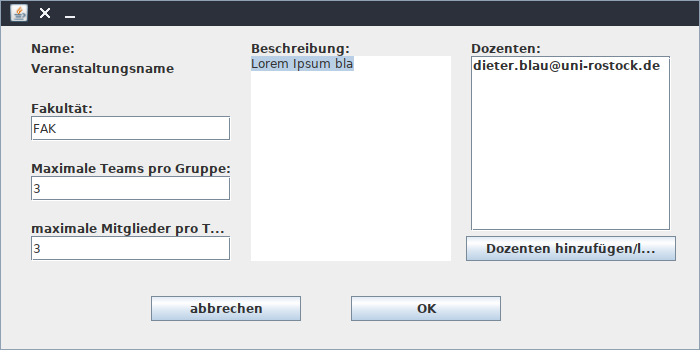
\includegraphics[width=0.7\textwidth]{img_adminGUI_09.png}
\end{center}
Jetzt könne sie mit \frqq OK\flqq{} Ihre Änderungen bestätigen und diese werden in das System übernommen.
\begin{center}
	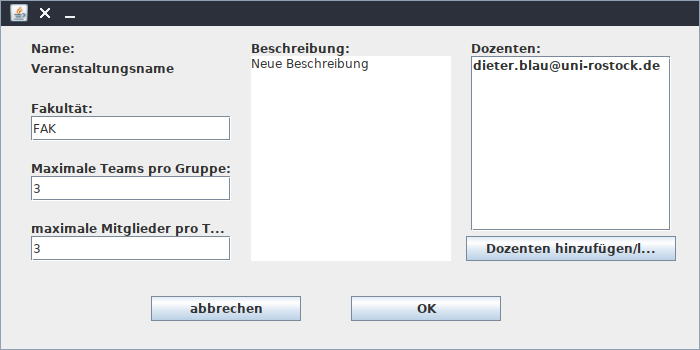
\includegraphics[width=0.7\textwidth]{img_adminGUI_10.png}
\end{center}

\subsection{Veranstaltung löschen}
Um eine Veranstaltung zu löschen, wählen Sie die zu löschenden Veranstaltung aus.
\begin{center}
	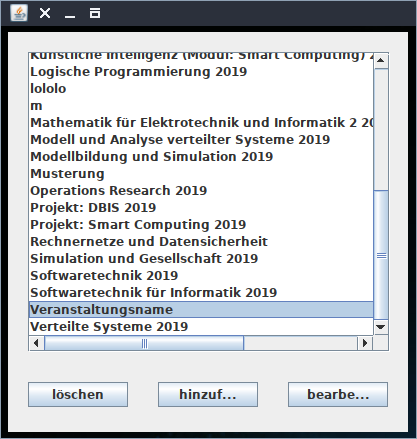
\includegraphics[width=0.7\textwidth]{img_adminGUI_11.png}
\end{center}
Klicken Sie auf den \frqq löschen\flqq{} Button. Achten Sie dabei darauf, dass es keine weitere Abfrage gibt, ob Sie diese Veranstaltung wirklich löschen wollen. Wir halten von solchen nervigen Mehrfachbestätigungen nichts und gehen davon aus, dass Sie wissen, was Sie wollen, und sich der Konsequenzen Ihres Handelns bewusst sind.
\begin{center}
	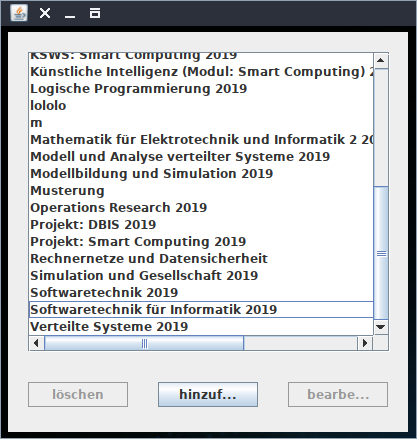
\includegraphics[width=0.7\textwidth]{img_adminGUI_12.png}
\end{center}
Das waren alle Funktionen des Admin Tools zur Verwaltung der Veranstaltungen.




%%%%%%%%%%%%%%%%%%%%%%%%%%%%%%%%%%%%
\newpage
\section{Dozentenhandbuch}
Beim Starten der Anwendung besteht die Möglichkeit, sich in der Software neu zu registrieren, oder sich mit einem bestehenden Account einzuloggen.

\subsection{Registrierung}
Um sich neu zu registrieren, klicken Sie auf der Login-Seite den Button \frqq Registrieren\flqq{}. 
\begin{center}
	\includegraphics[width=0.7\textwidth]{img_DozentenGUI_01.png}
\end{center}
Dann erscheint ein Fenster, in dem Sie Ihre persönlichen Daten eingeben können. 
\begin{center}
	\includegraphics[width=0.7\textwidth]{img_DozentenGUI_02.png}
\end{center}
Wählen Sie die Rolle \glqq Dozent\grqq{} und füllen Sie die restlichen Eingabefelder aus (Angabe des Titels ist optional.) Bitte geben Sie im Feld \glqq E-Mailadresse\grqq{} nur den ersten Teil Ihrer Universitätsmailadresse an.
\begin{center}
	\includegraphics[width=0.7\textwidth]{img_DozentenGUI_03.png}
\end{center}
Klicken Sie auf \frqq Verifizieren\flqq. 
\begin{center}
	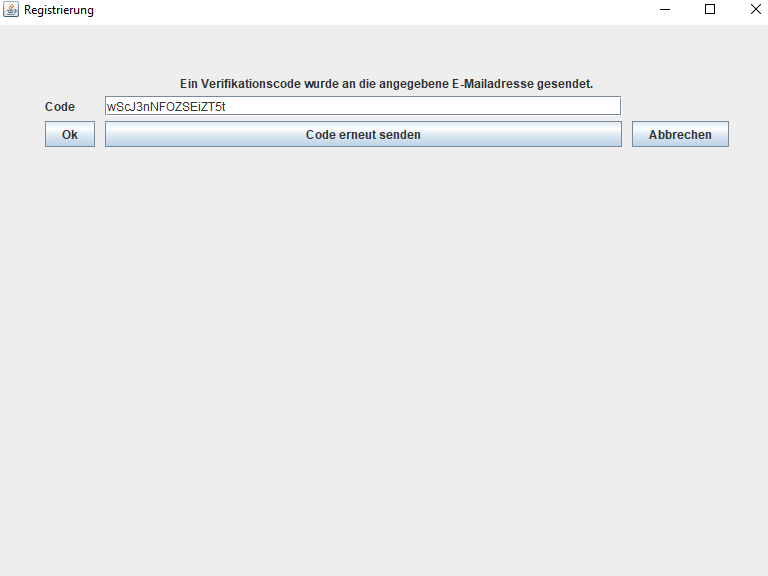
\includegraphics[width=0.7\textwidth]{img_DozentenGUI_04.png}
\end{center}
Nun erscheint ein Fenster zur Verifizierung und es wird ein Bestätigungscode an ihre Universitätsmailadresse gesendet. Fügen Sie diesen in das Feld ein und klicken Sie auf \frqq OK\flqq.
Falls Sie keine E-Mail erhalten haben sollten, klicken Sie auf \frqq Code erneut senden\flqq. 

\subsection{Login}
Wenn Sie bereits einen Account besitzen, geben Sie nach Start der Anwendung ihre E-Mail und Passwort ein und klicken Sie auf \frqq Login\flqq. 
\begin{center}
	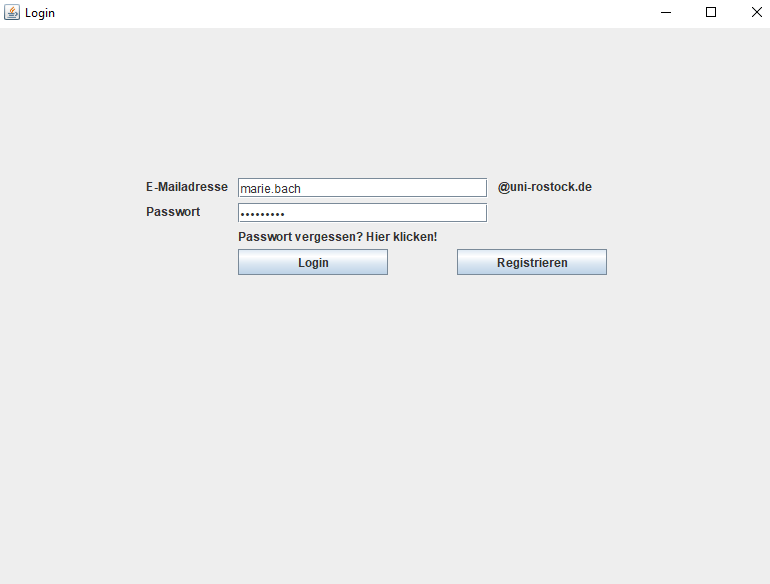
\includegraphics[width=0.7\textwidth]{img_DozentenGUI_05.png}
\end{center}Dann werden Sie zur Übersicht aller Veranstaltungen weitergeleitet, für die Sie verantwortlich sind. Um zusätzlichen Veranstaltungen zugewiesen zu werden oder neue Veranstaltungen zu erstellen, wenden Sie sich bitte an den Administrator.

\subsection{Passwort wiederherstellen und ändern}
Falls Sie Ihr Passwort vergessen haben, können Sie auf der Login-Seite ein neues Passwort anfordern.
\begin{center}
	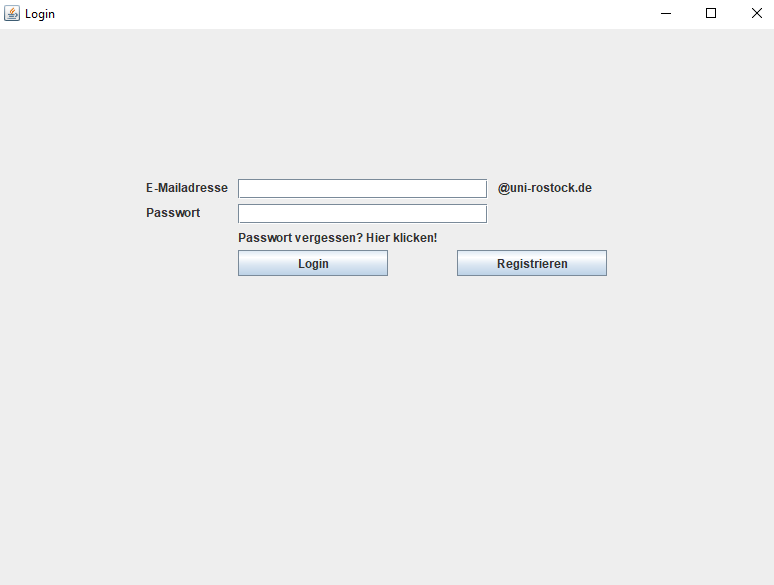
\includegraphics[width=0.7\textwidth]{img_DozentenGUI_06.png}
\end{center}
 Klicken Sie hierfür auf \frqq Passwort vergessen? Hier klicken!\flqq. 
 \begin{center}
	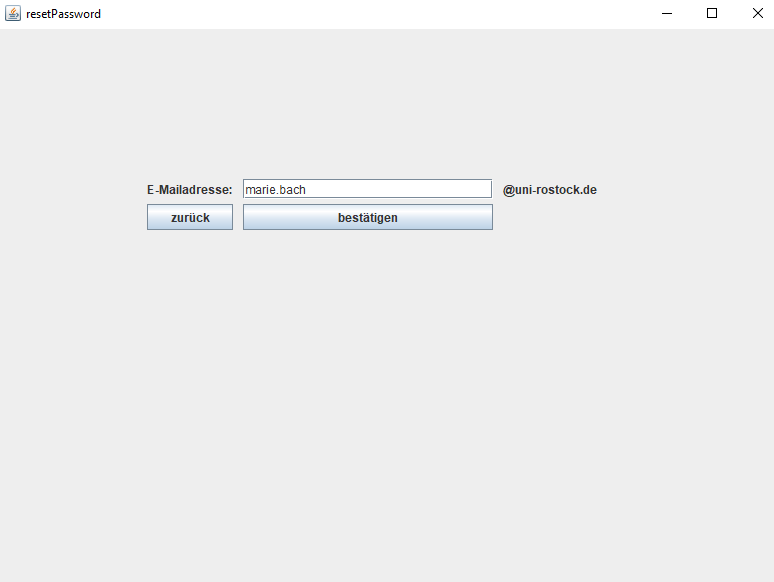
\includegraphics[width=0.7\textwidth]{img_DozentenGUI_07.png}
\end{center}
Geben Sie im Feld \glqq E-Mailadresse\grqq{} die E-Mailadresse an, die Sie zur Registrierung verwendet haben. Das System sendet Ihnen dann ein neues Passwort zu, mit dem Sie sich wieder anmelden können.

\subsection{Veranstaltungen einsehen und bearbeiten}
\begin{center}
	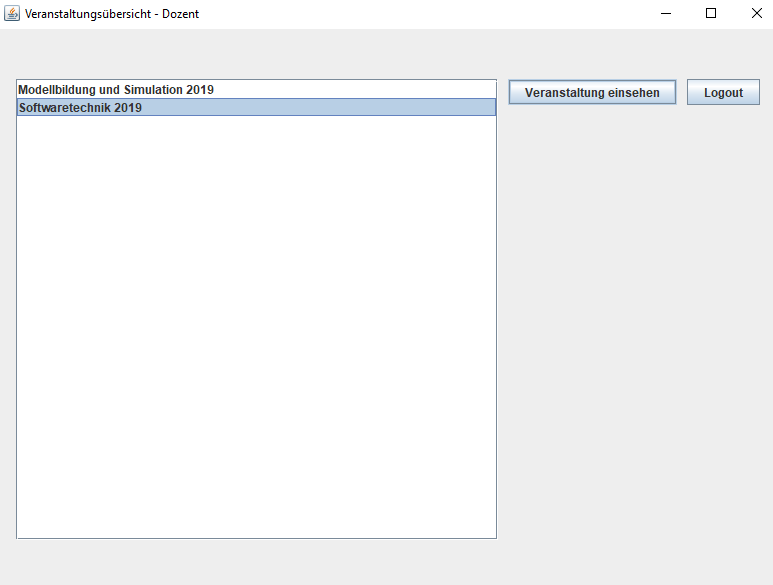
\includegraphics[width=0.7\textwidth]{img_DozentenGUI_08.png}
\end{center}
Markieren Sie eine Veranstaltung aus der Liste ihrer Veranstaltungen aus und klicken Sie \frqq Veranstaltung einsehen\flqq. Dann werden Sie zur Detailübersicht der markierten Veranstaltung weitergeleitet. 
\begin{center}
	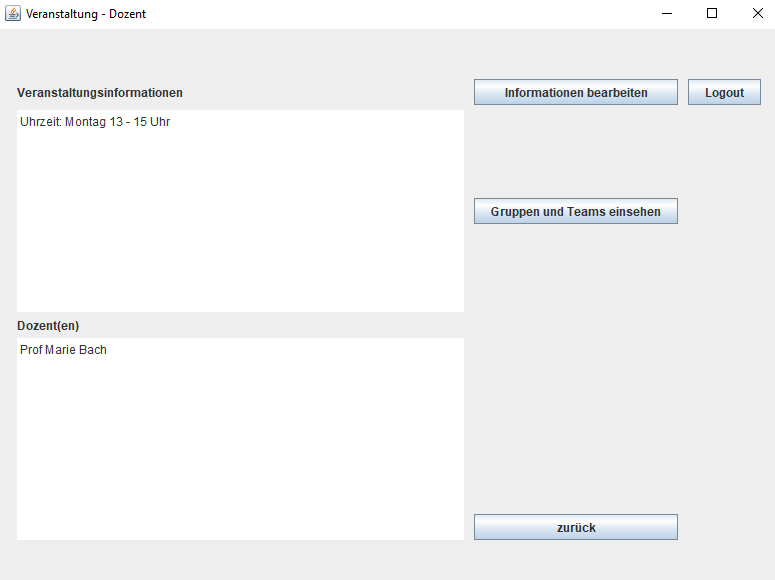
\includegraphics[width=0.7\textwidth]{img_DozentenGUI_09.png}
\end{center}
Hier sehen Sie Informationen zur Veranstaltung und die Liste der zuständigen Dozenten. Mit einem Klick auf \frqq Informationen bearbeiten\flqq{} wird das Feld der Veranstaltungsinformationen interaktiv und Sie können den Informationstext verändern. Um Ihre Änderungen ins System zu übernehmen, klicken Sie auf \frqq Änderungen bestätigen\flqq.

\subsection{Gruppen und Teams einsehen und verwalten}
Aus der Detailansicht einer Veranstaltung gelangen Sie durch Klick auf \frqq Gruppen und Teams einsehen\flqq{} in die Gruppenübersicht der Veranstaltung. 
\begin{center}
	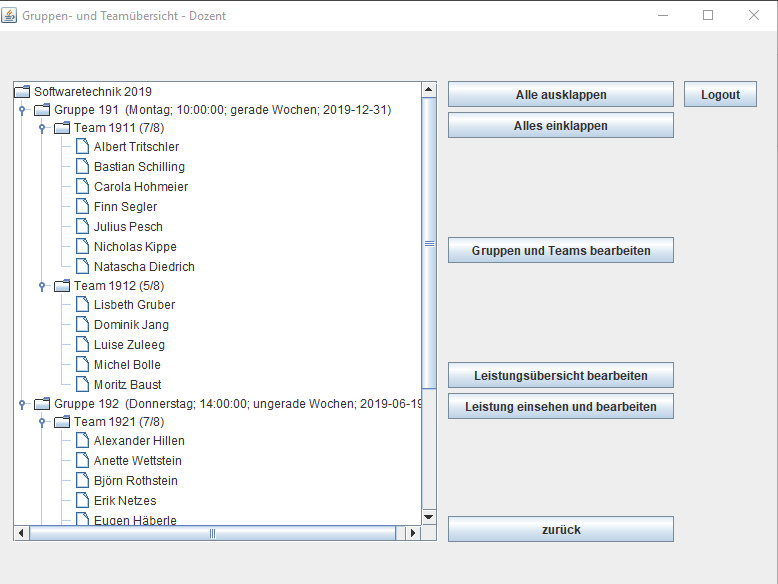
\includegraphics[width=0.7\textwidth]{img_DozentenGUI_11.png}
\end{center}Dort werden ihnen alle Übungsgruppen, die untergeordneten Projektteams und deren Mitglieder angezeigt. Mit einem Klick auf \frqq Gruppen und Teams bearbeiten\flqq{} gelangen Sie in die Bearbeitungsansicht. 
\begin{center}
	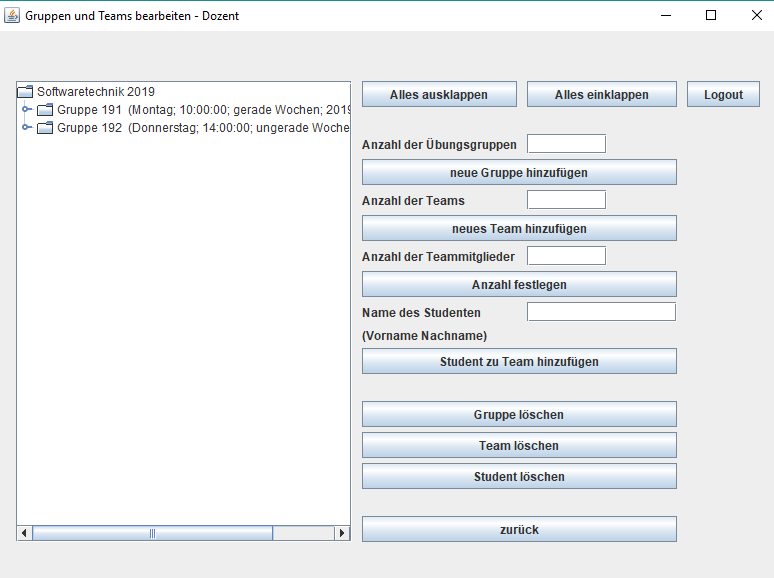
\includegraphics[width=0.7\textwidth]{img_DozentenGUI_12.png}
\end{center}
Hier können Sie Gruppen und Teams erstellen und löschen, die Maximalzahl der Teammitglieder festlegen und Studenten zu Teams hinzufügen und entfernen.\\
Um Übungsgruppen zu erstellen, geben Sie unter \glqq Anzahl der Übungsgruppen\grqq{} die Anzahl der Gruppen ein, die Sie erstellen wollen, und klicken Sie dann auf \frqq neue Gruppe hinzufügen\flqq. 
\begin{center}
	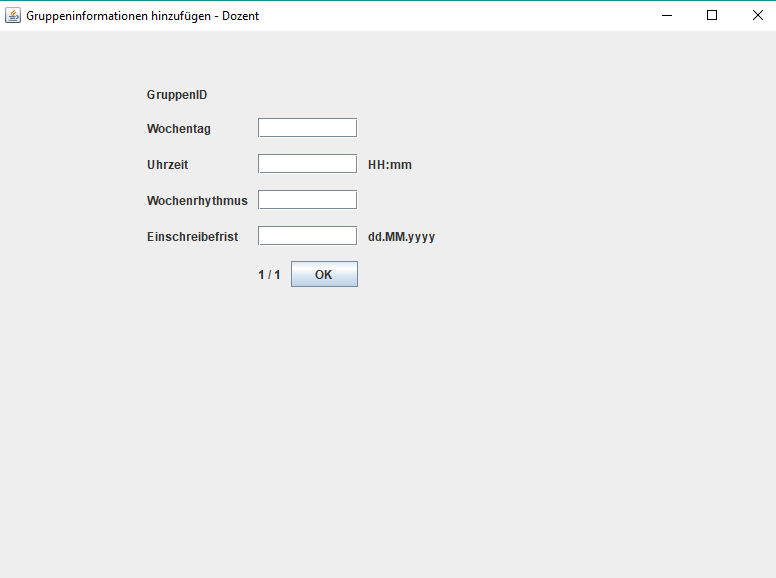
\includegraphics[width=0.7\textwidth]{img_DozentenGUI_13.png}
\end{center}Es öffnet sich eine neue Ansicht, in dem Sie Wochentag, Uhrzeit, Wochenrhythmus und Einschreibefrist für jede zu erstellende Gruppe eingeben müssen. Klicken Sie auf \frqq OK\flqq{} um ihre Eingaben zu bestätigen und die Gruppe zu erstellen. \\
Um Projektteams zu erstellen, wählen Sie die Gruppe aus, in der das neue Team erstellt werden soll. Geben Sie unter \glqq Anzahl der Teams\grqq{} die Anzahl der Projektteams ein, die Sie erstellen wollen, und klicken Sie dann auf \frqq neues Team hinzufügen\flqq. 
\begin{center}
	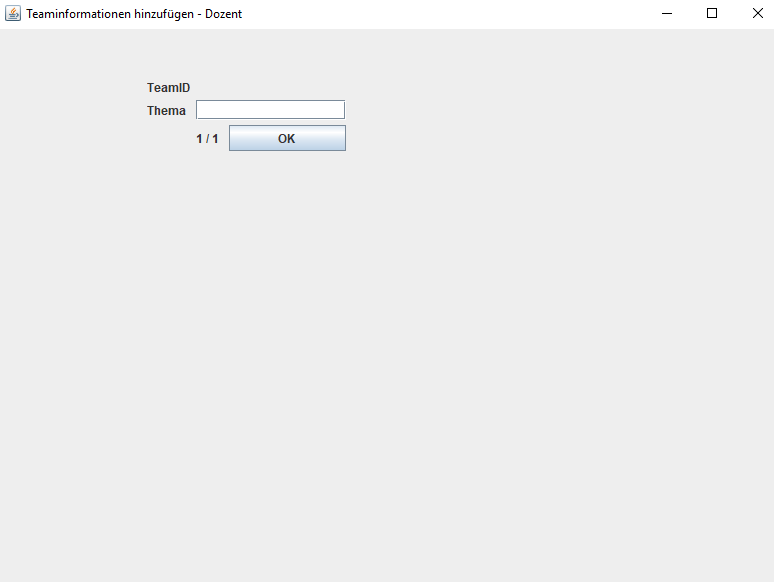
\includegraphics[width=0.7\textwidth]{img_DozentenGUI_14.png}
\end{center}Es öffnet sich eine neue Ansicht, in der Sie jedem Team ein eigenes Thema zuweisen können. Klicken Sie auf \frqq OK\flqq{} um ihre Eingaben zu bestätigen und das Team zu erstellen. \\
Um die maximale Anzahl der Teammitglieder anzupassen, wählen Sie das zu bearbeitende Team aus, geben Sie die gewünschte Anzahl unter  \glqq Anzahl der Teammitglieder\grqq{} ein und klicken sie auf \frqq Anzahl festlegen\flqq.\\
Um einem Team ein neues Mitglied hinzuzufügen, geben Sie Vor- und Nachname des gewünschten Mitglieds unter \glqq Name des Studenten\grqq{} ein und klicken Sie auf \frqq Student zu Team hinzufügen\flqq.\\
Um Gruppen zu löschen, wählen Sie die zu löschende Gruppe aus und klicken Sie auf \frqq Gruppe löschen\flqq.\\
Um Teams zu löschen, wählen Sie das zu löschende Team aus und klicken Sie auf \frqq Team löschen\flqq.\\
Um Studenten aus einem Team zu entfernen, wählen Sie den zu löschenden Studenten aus und klicken Sie auf \frqq Student löschen\flqq.\\

\subsection{Leistungen erstellen und verwalten}
Um einer Veranstaltung Leistungen hinzuzufügen, wechseln Sie in die Gruppenübersicht der gewünschten Veranstaltung und klicken Sie auf \frqq Leistungsübersicht bearbeiten\flqq. Hier können Sie Leistungen, Unterblöcke und Aufgaben erstellen.
\begin{center}
	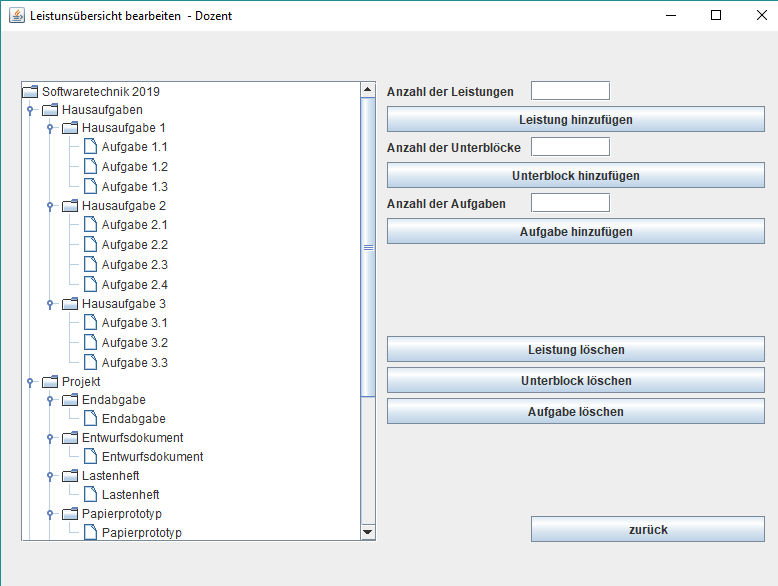
\includegraphics[width=0.7\textwidth]{img_DozentenGUI_15.png}
\end{center}
Um Leistungen zu erstellen, geben Sie unter \glqq Anzahl der Leistungen\grqq{} die Anzahl der Leistungen ein, die Sie erstellen wollen, und klicken Sie dann auf \frqq Leistung hinzufügen\flqq. 
\begin{center}
	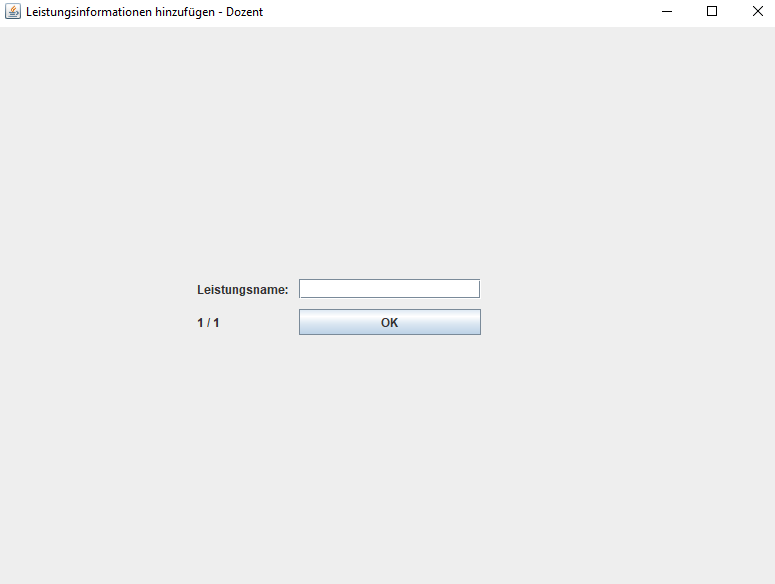
\includegraphics[width=0.7\textwidth]{img_DozentenGUI_16.png}
\end{center}
Es öffnet sich eine neue Ansicht, in der Sie jede Leistung benennen können. Klicken Sie auf \frqq OK\flqq{} um ihre Eingaben zu bestätigen und die Leistung zu erstellen. \\
Um Unterblöcke zu erstellen, wählen Sie die Leistung aus, in der der neue Unterblock erstellt werden soll. Geben Sie unter \glqq Anzahl der Unterblöcke\grqq{} die Anzahl der Unterblöcke ein, die Sie erstellen wollen, und klicken Sie dann auf \frqq Unterblock hinzufügen\flqq. 
\begin{center}
	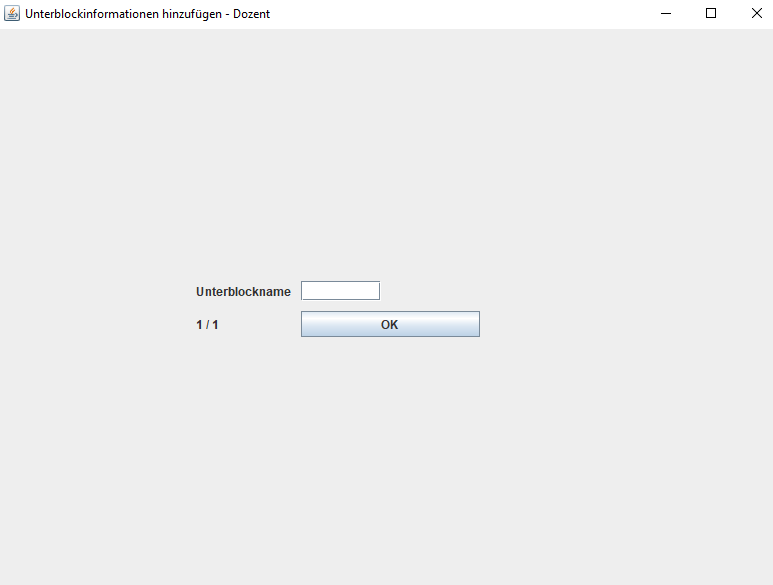
\includegraphics[width=0.7\textwidth]{img_DozentenGUI_17.png}
\end{center}
Es öffnet sich eine neue Ansicht, in der Sie jedem Unterblock bennenen können. Klicken Sie auf \frqq OK\flqq{} um ihre Eingaben zu bestätigen und den Unterblock zu erstellen. \\
Um Aufgaben zu erstellen, wählen Sie den Unterblock aus, in dem die neue Aufgabe erstellt werden soll. Geben Sie unter \glqq Anzahl der Aufgaben\grqq{} die Anzahl der Aufgaben ein, die Sie erstellen wollen, und klicken Sie dann auf \frqq Aufgabe hinzufügen\flqq. 
\begin{center}
	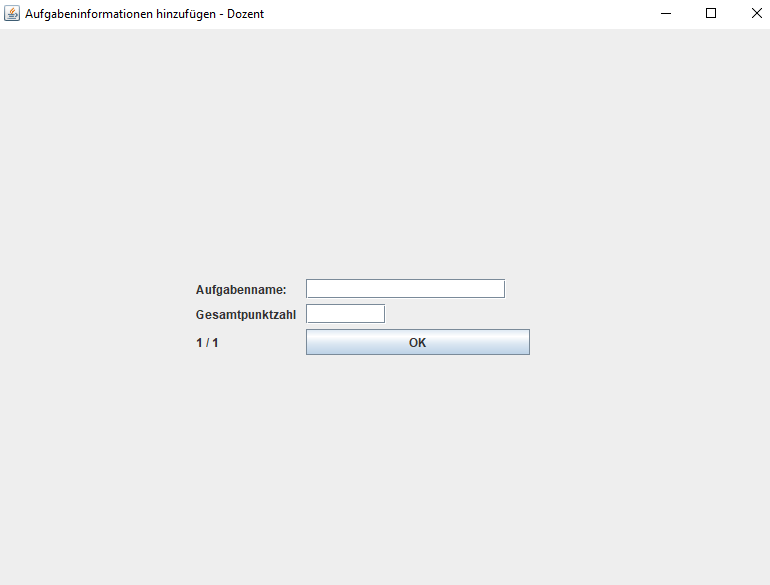
\includegraphics[width=0.7\textwidth]{img_DozentenGUI_18.png}
\end{center}
Es öffnet sich eine neue Ansicht, in der Sie jede Aufgabe bennenen und ihre Gesamtpunktzahl eingeben können. Klicken Sie auf \frqq OK\flqq{} um ihre Eingaben zu bestätigen und die Aufgabe zu erstellen.\\
Um Leistungen zu löschen, wählen Sie die zu löschende Leistung aus und klicken Sie auf \frqq Leistung löschen\flqq.\\
Um Unterblöcke zu löschen, wählen Sie den zu löschenden Unterblock aus und klicken Sie auf \frqq Unterblock löschen\flqq.\\
Um Aufgaben zu löschen, wählen Sie die zu löschende Aufgabe aus und klicken Sie auf \frqq Aufgabe löschen\flqq.\\

\subsection{Leistungsbewertungen erstellen und verwalten}
\begin{center}
	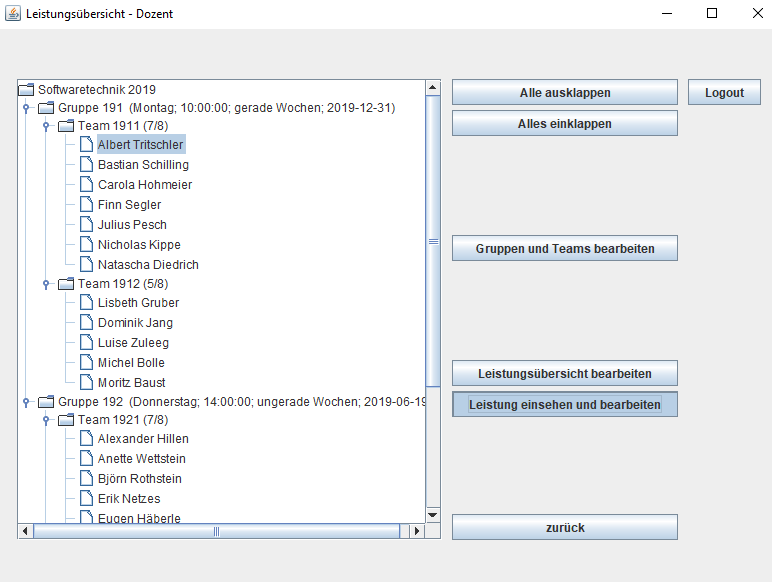
\includegraphics[width=0.7\textwidth]{img_DozentenGUI_19.png}
\end{center}
Um die Leistungen von Teams und Studenten zu bewerten, wechseln Sie in die Gruppenübersicht der gewünschten Veranstaltung, wählen Sie den gewünschten Studenten (zur Bewertung von Teamleistungen reicht ein beliebiger Student des Teams) und klicken Sie auf \frqq Leistung einsehen und bearbeiten\flqq. 
\begin{center}
	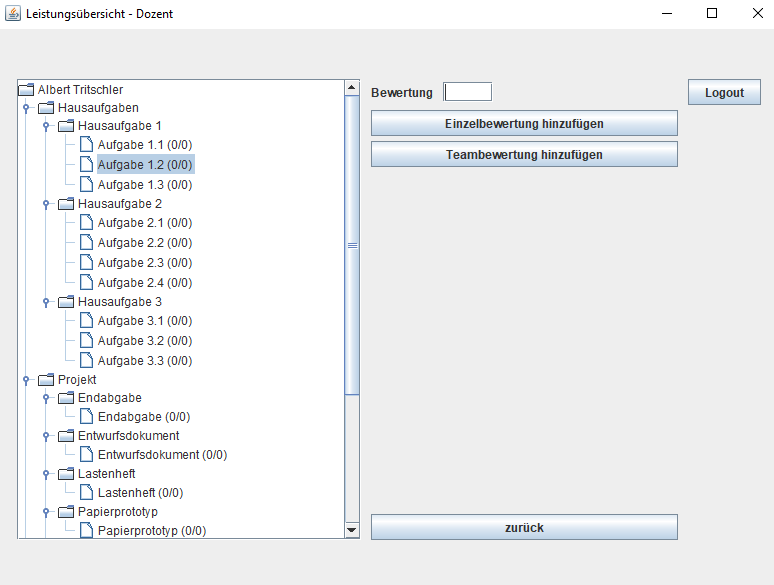
\includegraphics[width=0.7\textwidth]{img_DozentenGUI_20.png}
\end{center}
Um eine Individualleistung zu bewerten, wählen Sie die zu bewertende Aufgabe aus der Übersicht aus, geben Sie unter \glqq Bewertung\grqq{} die erreichten Punkte ein und klicken Sie auf \frqq Einzelbewertung hinzufügen\flqq.\\
Um eine Teamleistung zu bewerten, wählen Sie die zu bewertende Aufgabe aus der Übersicht aus, geben Sie unter \glqq Bewertung\grqq{} die erreichten Punkte ein und klicken Sie auf \frqq Teambewertung hinzufügen\flqq. Dadurch wird die Bewertung automatisch bei allen Teammitgliedern eingetragen. 


\subsection{Logout}
Mit dem Button \frqq Logout\flqq{} können Sie sich jederzeit aus dem System ausloggen.


%%%%%%%%%%%%%%%%%%%%%%%%%%%%%%%%%%%%
\newpage
\section{Studentenhandbuch}
Beim Starten der Anwendung besteht die Möglichkeit, sich in der Software neu zu registrieren, oder sich mit einem bestehenden Account einzuloggen.

\subsection{Registrierung}
Um sich neu zu registrieren, klicken Sie auf der Login-Seite den Button \frqq Registrieren\flqq{}. 
\begin{center}
	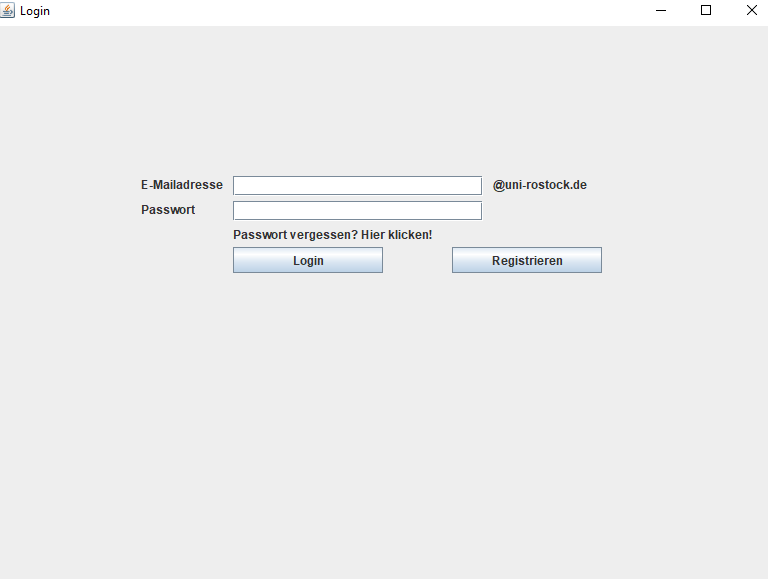
\includegraphics[width=0.7\textwidth]{student00.png}
\end{center}
Dann erscheint ein Fenster, in dem Sie Ihre persönlichen Daten eingeben können. 
\begin{center}
	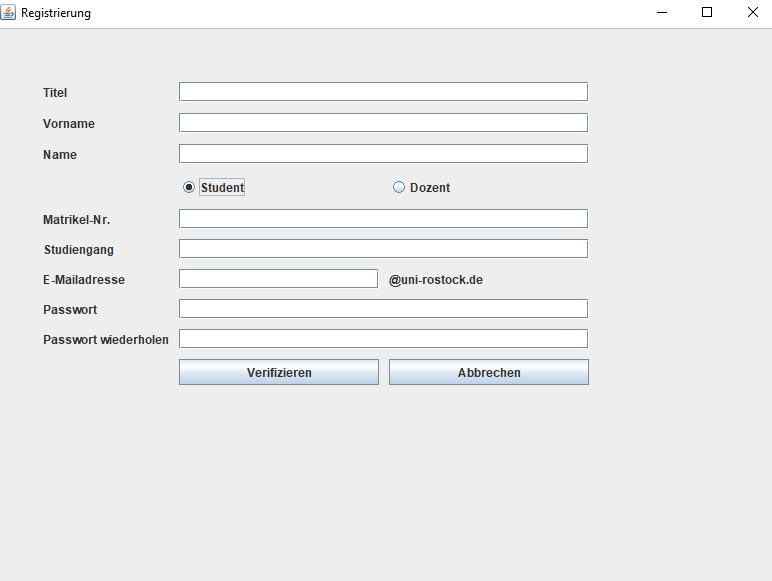
\includegraphics[width=0.7\textwidth]{student02.png}
\end{center}
Wählen Sie die Rolle \glqq Student\grqq{} und füllen Sie die restlichen Eingabefelder aus (Angabe des Titels ist optional.) Bitte geben Sie im Feld \glqq E-Mailadresse\grqq{} nur den ersten Teil Ihrer Universitätsmailadresse an.
Klicken Sie auf \frqq Verifizieren\flqq. 
\begin{center}
	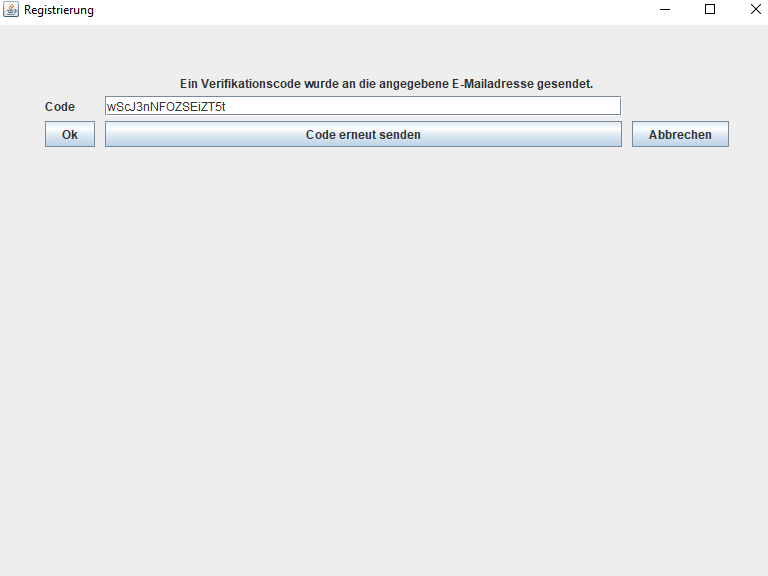
\includegraphics[width=0.7\textwidth]{img_DozentenGUI_04.png}
\end{center}
Nun erscheint ein Fenster zur Verifizierung und es wird ein Bestätigungscode an ihre Universitätsmailadresse gesendet. Fügen Sie diesen in das Feld ein und klicken Sie auf \frqq OK\flqq.
Falls Sie keine E-Mail erhalten haben sollten, klicken Sie auf \frqq Code erneut senden\flqq. 

\subsection{Login}
Wenn Sie bereits einen Account besitzen, geben Sie nach Start der Anwendung ihre E-Mail und Passwort ein und klicken Sie auf \frqq Login\flqq. Dann werden Sie zur Übersicht aller Veranstaltungen weitergeleitet, in die Sie derzeit eingeschrieben sind. 

\subsection{Passwort wiederherstellen und ändern}
\begin{center}
	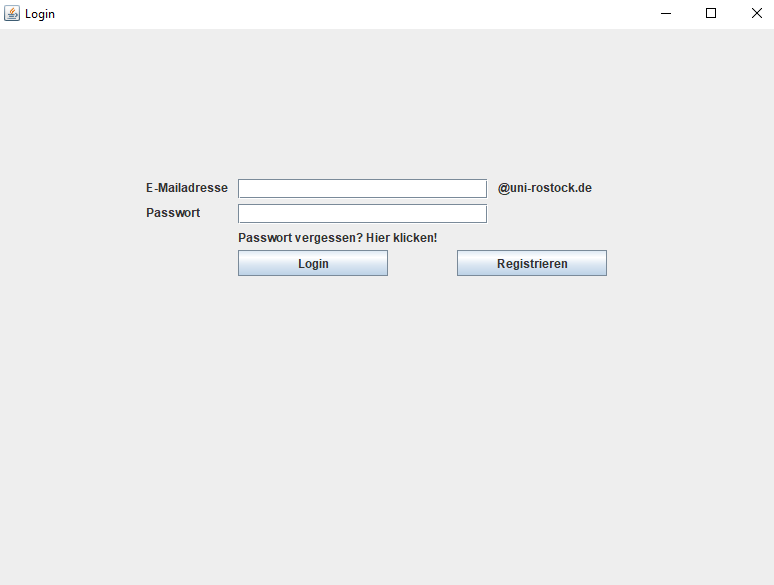
\includegraphics[width=0.7\textwidth]{img_DozentenGUI_06.png}
\end{center}
Falls Sie Ihr Passwort vergessen haben, können Sie auf der Login-Seite ein neues Passwort anfordern. Klicken Sie hierfür auf \frqq Passwort vergessen? Hier klicken!\flqq. 
\begin{center}
	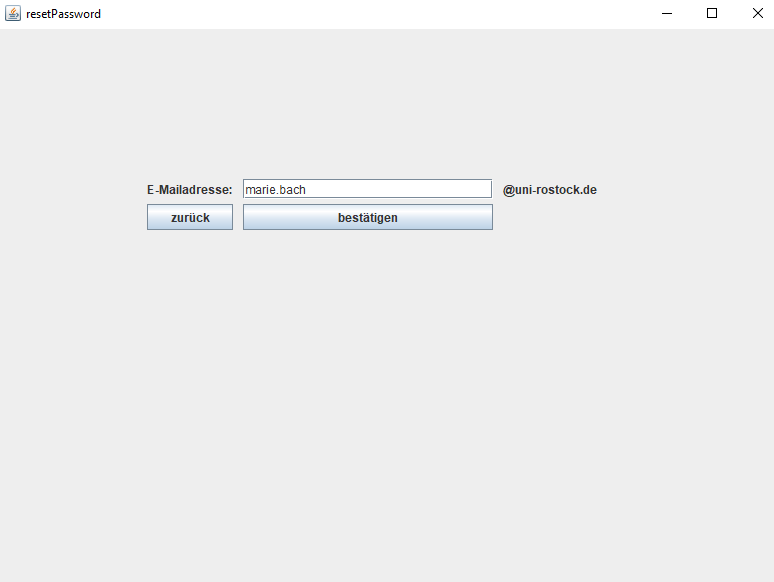
\includegraphics[width=0.7\textwidth]{img_DozentenGUI_07.png}
\end{center}
Geben Sie im Feld \glqq E-Mailadresse\grqq{} die E-Mailadresse an, die Sie zur Registrierung verwendet haben. Das System sendet Ihnen dann ein neues Passwort zu, mit dem Sie sich wieder anmelden können. 
Um Ihr Passwort zu ändern, loggen Sie sich mit Ihrem alten Passwort ein. In der Veranstaltungsübersicht klicken Sie auf \frqq Passwort ändern\flqq. Geben Sie Ihr altes Passwort ein und wählen Sie ein neues Passwort. Klicken Sie auf \frqq bestätigen\flqq{} um ihr neues Passwort zu speichern.

\subsection{Veranstaltung hinzufügen/verlassen}
Um einer Veranstaltung beizutreten, klicken Sie auf \frqq Veranstaltung hinzufügen\flqq{}. 
\begin{center}
	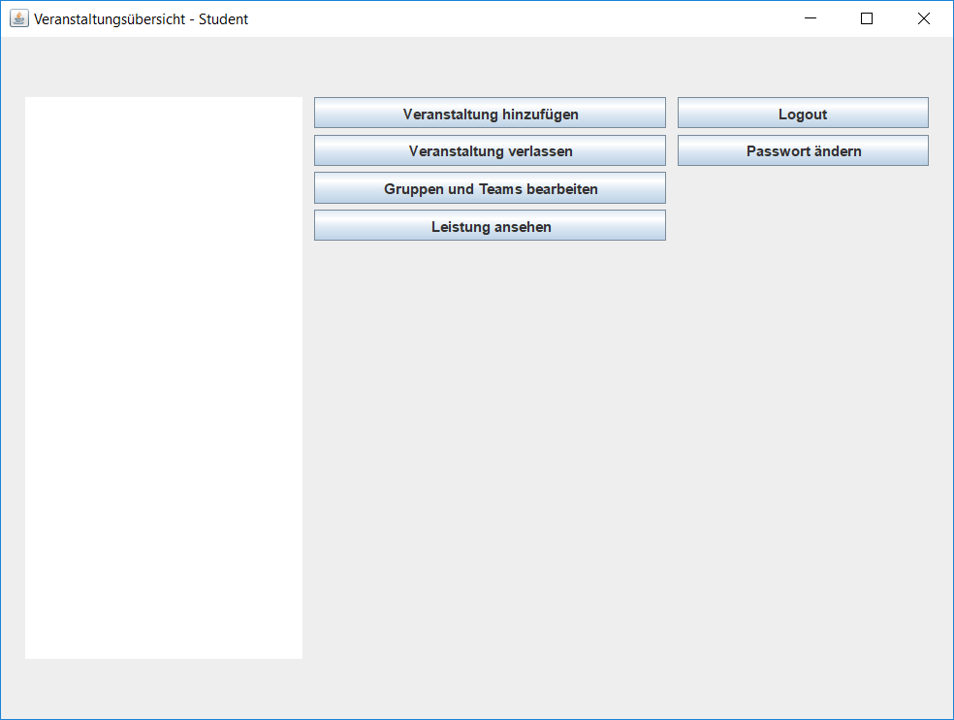
\includegraphics[width=0.7\textwidth]{img_student1.jpg}
\end{center}
In der nun angezeigten Veranstaltungsübersicht werden alle verfügbaren Veranstaltungen in einer Liste angezeigt. Aus dieser wählen Sie die gewünschte Veranstaltung und klicken auf \frqq in Veranstaltung eintragen\flqq{}.
\begin{center}
	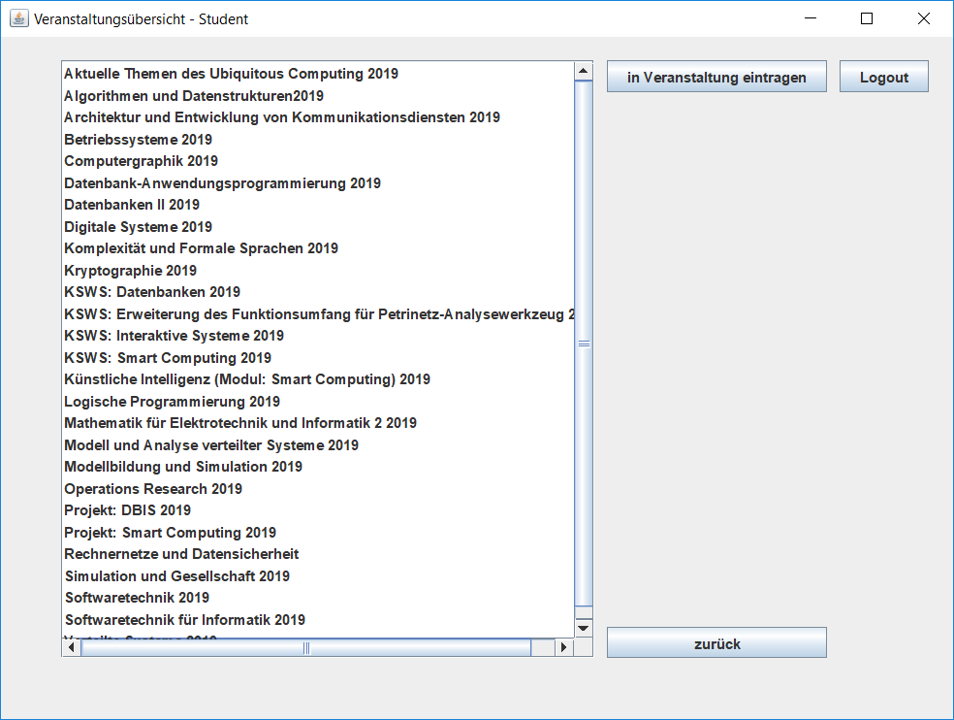
\includegraphics[width=0.7\textwidth]{img_student2.jpg}
\end{center}
Anschließend wird eine Gruppenübersicht mit allen Übungsgruppen und Teams angezeigt. Um sich abschließend in die Veranstaltung einzutragen, müssen Sie sich noch in ein Team eintragen. (Siehe Sektion \ref{sec:gruppenteamsbearbeiten})
Erst jetzt wird die Änderung im System übernommen.
Sie können jederzeit mit dem Button \frqq zurück\flqq{} in das Hauptmenü gelangen. Um die Veranstaltungsliste im Hauptmenü zu aktualisieren, müssen Sie sich aus- und wieder einloggen.
Die nun im Hauptmenü angezeigten Veranstaltungen können Sie wieder verlassen, indem Sie die jeweilige Veranstaltung in der Liste auswählen und auf \frqq Veranstaltung verlassen\flqq{} klicken. 

\subsection{Gruppen und Teams bearbeiten}\label{sec:gruppenteamsbearbeiten}
Um die Gruppen und Teams einer Veranstaltung zu bearbeiten wählen Sie die jeweilige Veranstaltung im Hauptmenü aus und klicken auf \frqq Gruppen und Teams bearbeiten\flqq{}.
Nun sind Sie in der Gruppenübersicht. Sie können einem Team beitreten, indem Sie es in der links angezeigten Liste auswählen und auf \frqq Team beitreten\flqq{} klicken. 
\begin{center}
	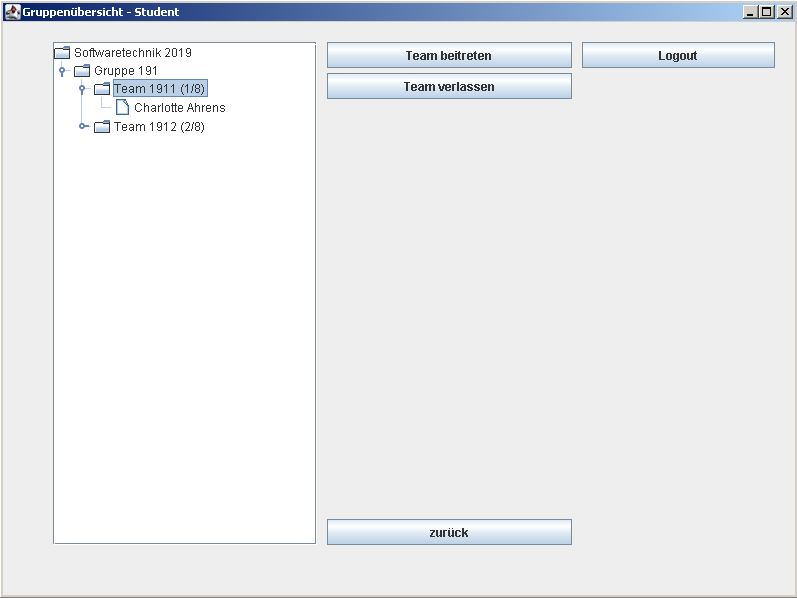
\includegraphics[width=0.7\textwidth]{img_student3.jpg}
\end{center}
Mit dem Button \frqq Team verlassen\flqq{} können Sie sich wieder aus einem Team austragen.

\subsection{Leistungen ansehen}
\begin{center}
	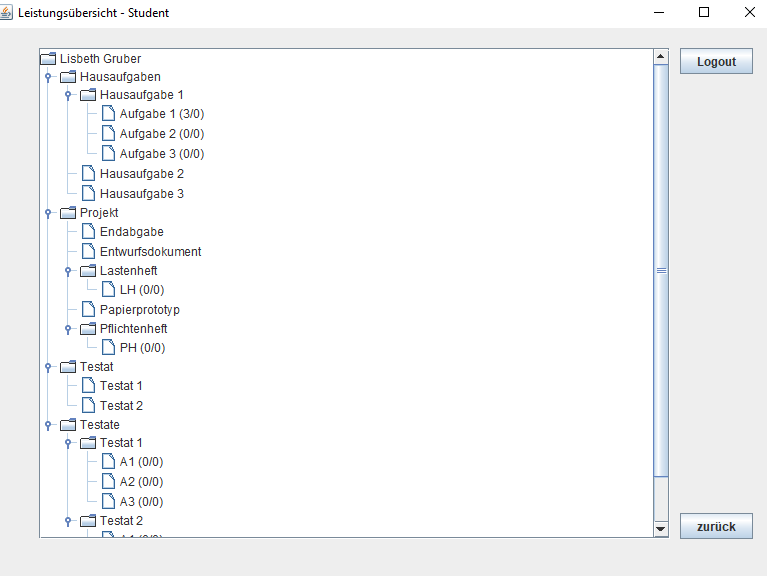
\includegraphics[width=0.7\textwidth]{student4.png}
\end{center}
Ihre erreichten Leistungen in einer Veranstaltung können sie überprüfen, indem Sie die gewünschte Veranstaltung auswählen und auf \frqq Leistungen ansehen\flqq{} klicken.


\subsection{Logout}
Mit dem Button \frqq Logout\flqq{} können Sie sich jederzeit aus dem System ausloggen.



\end{document}



\begin{center}
	\includegraphics[width=0.7\textwidth]{}
\end{center}